\documentclass{article}

\usepackage[margin=2.5cm,left=2cm,includefoot]{geometry}
\usepackage{graphicx}
\usepackage{float}
\usepackage[space]{grffile}
\usepackage{hyperref}
\usepackage[export]{adjustbox}
\usepackage{multicol}
\usepackage{caption}
\usepackage{hyperref}
\usepackage{listings}
\newcommand{\nexists}{\not\exists}
\newcommand\tab[1][0.5cm]{\hspace*{#1}}

\usepackage{tabulary}
\newcolumntype{K}[1]{>{\centering\arraybackslash}p{#1}}


\usepackage{titlesec}

\setcounter{secnumdepth}{4}

\titleformat{\paragraph}
{\normalfont\normalsize\bfseries}{\theparagraph}{1em}{}
\titlespacing*{\paragraph}
{0pt}{3.25ex plus 1ex minus .2ex}{1.5ex plus .2ex}

% Header and footer
\usepackage{fancyhdr}
\pagestyle{fancy}

\rhead{COS301}
\lhead{Functional Specification}
\fancyfoot[R]{Page \thepage}

\renewcommand{\headrulewidth}{2pt}
\renewcommand{\footrulewidth}{1pt}

\begin{document}

	\begin{titlepage}
		\begin{center}
			
\includegraphics[width=10cm]{images/UP.jpg}  \\
			[0.5cm]
			\huge{
			Functional Specification\\
			}

			\line(1,0){300}\\
			[0.2cm]
			\LARGE{Project: Insurance profiling from social media\\
			Client: RetroRabbit} \\
			\line(1,0){300}\\
			\LARGE{Team: Valknut Solutions}\\
			[1.0cm]
			\large
			{
			\begin{itemize}
				\item 13054903 - Charl Jansen van Vuuren
				\item 10297902 - Bernhard Schuld
				\item 13044924 - Kevin Heritage
				\item 13176545 - Quinton Weenink\\
			\end{itemize}
			}
			\textsc{\large}\\
		[3.0cm]
		\textsc{\large  Department of Computer Science}\\
		[0.5cm]
		\textsc{\large \today}\\
		\end{center}

		%\begin{figure}[H]}
		%\centering
		%\includegraphics[{imagename}
		%\end{figure}\

	\end{titlepage}
	\cleardoublepage
	\tableofcontents
	\cleardoublepage
\section{Version table}	

	\begin{table}[H]
	\centering
	\caption{Version Table}
	\label{my-label}
	\begin{tabular}{|l|l|l|l|l|}
	\hline
	version 	& build 	& description 		\\ \hline
	0.0.1		& \#45 		& Basic handlebars implementation with no api					\\
	0.0.2		& \#81 		& API routes and persistence working Facebook data still being implemented	\\ \hline
	\end{tabular}
	\end{table}

\section{Functional requirements and application design}
	\subsection{User subsystem}
		\subsubsection{Use cases}

		\begin{figure}[H]
		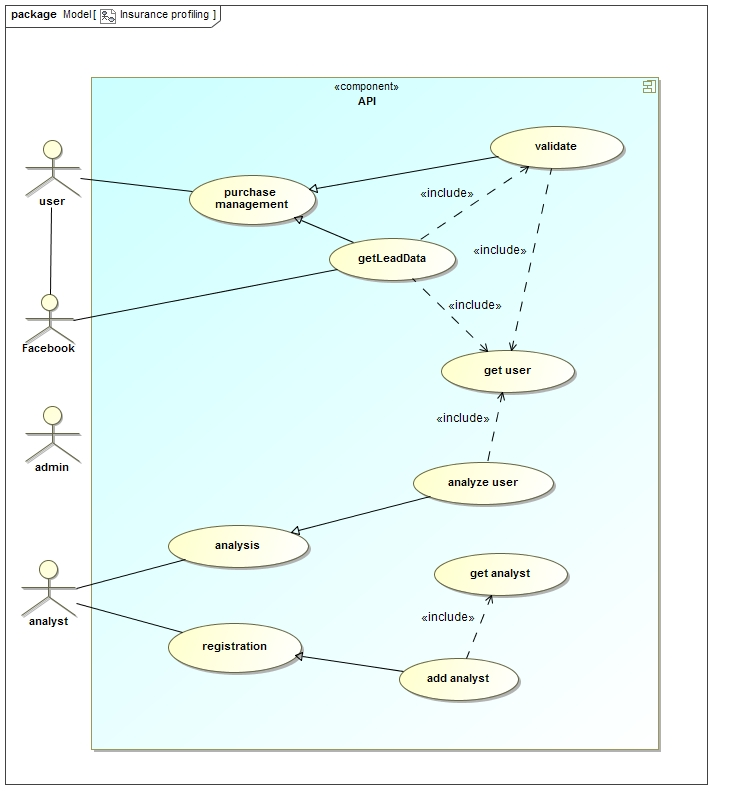
\includegraphics[width=\textwidth]{images/uc__Insurance_profiling.jpg}  \\
		\caption{Use Case Diagram : Publications}
		\end{figure}

		\begin{flushleft}
			\textbf{Critical}
				\begin{itemize}
	  				\item validateUser
	  				\item createUser
	  				\item getUser
				\end{itemize}
			\textbf{Important}
				\begin{itemize}
	  				\item validateUser
				\end{itemize}

			\textbf{Nice-To-Have}
				\begin{itemize}
	  				\item getAnalyst
	  				\item analiseUser
				\end{itemize}
		\end{flushleft}

		\subsubsection{Services Contracts}

		\begin{figure}[H]
		
\includegraphics[width=\textwidth]{images/Incomplete.png}  \\
		\caption{Use Case Diagram : Publications}
		\end{figure}

		\subsubsection{Required Functionality}

		\begin{figure}[H]
		
\includegraphics[width=\textwidth]{images/Incomplete.png}  \\
		\caption{Use Case Diagram : Publications}
		\end{figure}

		\subsubsection{Process specifications}

		\begin{figure}[H]
		
\includegraphics[width=\textwidth]{images/Incomplete.png}  \\
		\caption{Use Case Diagram : Publications}
		\end{figure}git 


	\subsection{Admin}

	\subsubsection{Use cases}

	\begin{figure}[H]
	
\includegraphics[width=\textwidth]{images/Incomplete.png}  \\
	\caption{Use Case Diagram : Publications}
	\end{figure}

		\begin{flushleft}
		\textbf{Critical}
			\begin{itemize}
					\item addPublication
					\item editPublication
					\item getPublication
					\item addPublicationStatus
					\item getPublicationStatus
					\item assignGoal
					\item unassignGoal
					\item accreditResearcher
					\item unaccreditResearcher
					\item linkGroup
					\item unlinkGroup
			\end{itemize}

		\textbf{Important}
			\begin{itemize}
					\item editPublicationStatus
					\item getPublicationProgression
					\item editPublicationProgression
					\item editPublicationStatus
			\end{itemize}

		\textbf{Nice-To-Have}
			\begin{itemize}
					\item getDepartmentPublications
					\item getGroupPublications
			\end{itemize}
	\end{flushleft}

	\subsubsection{Services Contracts}

	\begin{figure}[H]
	
\includegraphics[width=\textwidth]{images/Incomplete.png}  \\
	\caption{Use Case Diagram : Publications}
	\end{figure}

	\subsubsection{Required Functionality}

	\begin{figure}[H]
	
\includegraphics[width=\textwidth]{images/Incomplete.png}  \\
	\caption{Use Case Diagram : Publications}
	\end{figure}

	\subsubsection{Process specifications}

	\begin{figure}[H]
	
\includegraphics[width=\textwidth]{images/Incomplete.png}  \\
	\caption{Use Case Diagram : Publications}
	\end{figure}


\subsection{Domain model}

\begin{figure}[H]
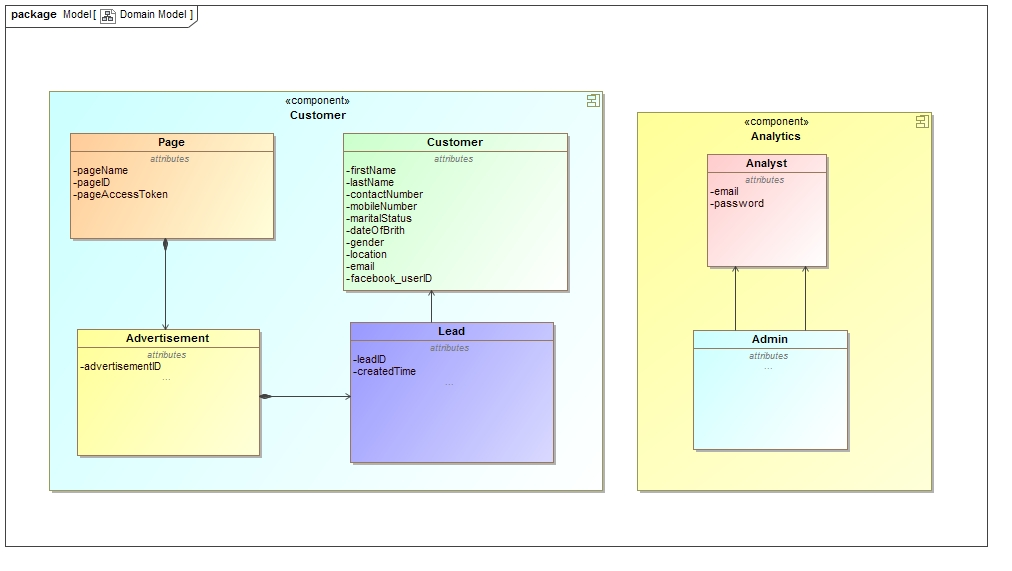
\includegraphics[width=\textwidth]{images/class__Domain_Model.jpg}  \\
\caption{Use Case Diagram : Publications}
\end{figure}

\subsection{Open Issues}






\end{document}
